\begin{figure}[H]
\begin{tabular}{@{}c@{}c@{}c@{}}
\begin{subfigure}[b]{0.30\textwidth}
\begin{center}
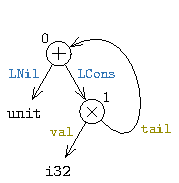
\includegraphics[scale=1.3]{chapters/figures/figTypeTreeList1.pdf}
\end{center}
\vspace{30px}
\caption{\label{fig:typetreelist1}\cons{List} = \cons{LNil} | \newline \cons{LCons}(\type{i32}, \type{List})}
\end{subfigure}%
&
\begin{subfigure}[b]{0.33\textwidth}
\begin{center}
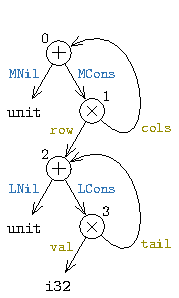
\includegraphics[scale=1.3]{chapters/figures/figTypeTreeMatrix1.pdf}
\end{center}
\caption{\label{fig:typetreematrix1}\cons{Matrix} = \cons{MNil} | \newline \cons{MCons}(\type{List}, \type{Matrix})}
\end{subfigure}%
&
\begin{subfigure}[b]{0.33\textwidth}
\begin{center}
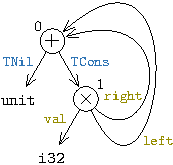
\includegraphics[scale=1.3]{chapters/figures/figTypeTreeTree1.pdf}
\end{center}
\caption{\label{fig:typetreetree1}\cons{Tree} = \cons{TNil} | \newline \cons{TCons}(\type{i32}, \type{Forest})}
\end{subfigure}%
\\
\end{tabular}
\caption{\label{fig:typetrees}Graphical representation for the types \type{List}, \type{Matrix} and \type{Tree}.}
\end{figure}